\chapter{Installation}

\textit{Covered in \href{https://www.youtube.com/watch?v=oIsH0V3fRt8&list=PLjGmdnqrOKuYXiu7lgG5HW71jPEUd1XCm&index=2}{video 1 of the series}}
\vspace{6mm}

Probably the most complicated installation procedure you have ever seen. However, it is only a one-time process. Those are essential tools for you to code more advanced stuff using JavaScript. It is also a good practice in using the command line interface.

\section*{For those of you not using Git}

You would still need to perform step 1: install Git Bash if you are using a Windows machine.\footnote{Because the Windows CMD uses slightly different command keywords.}

You can download the code as a zip file \href{https://github.com/KidProf/static-web-sandbox}{here}.\footnote{Link: \href{https://github.com/KidProf/static-web-sandbox}{https://github.com/KidProf/static-web-sandbox}}\textit{(see figure)} You do not need a GitHub account to do so. 

After that, proceed with step 5: Creating a folder using command line, and unzip your code inside the folder, then proceed with step 7: Installing node.js

\begin{figure}[h]
\centering
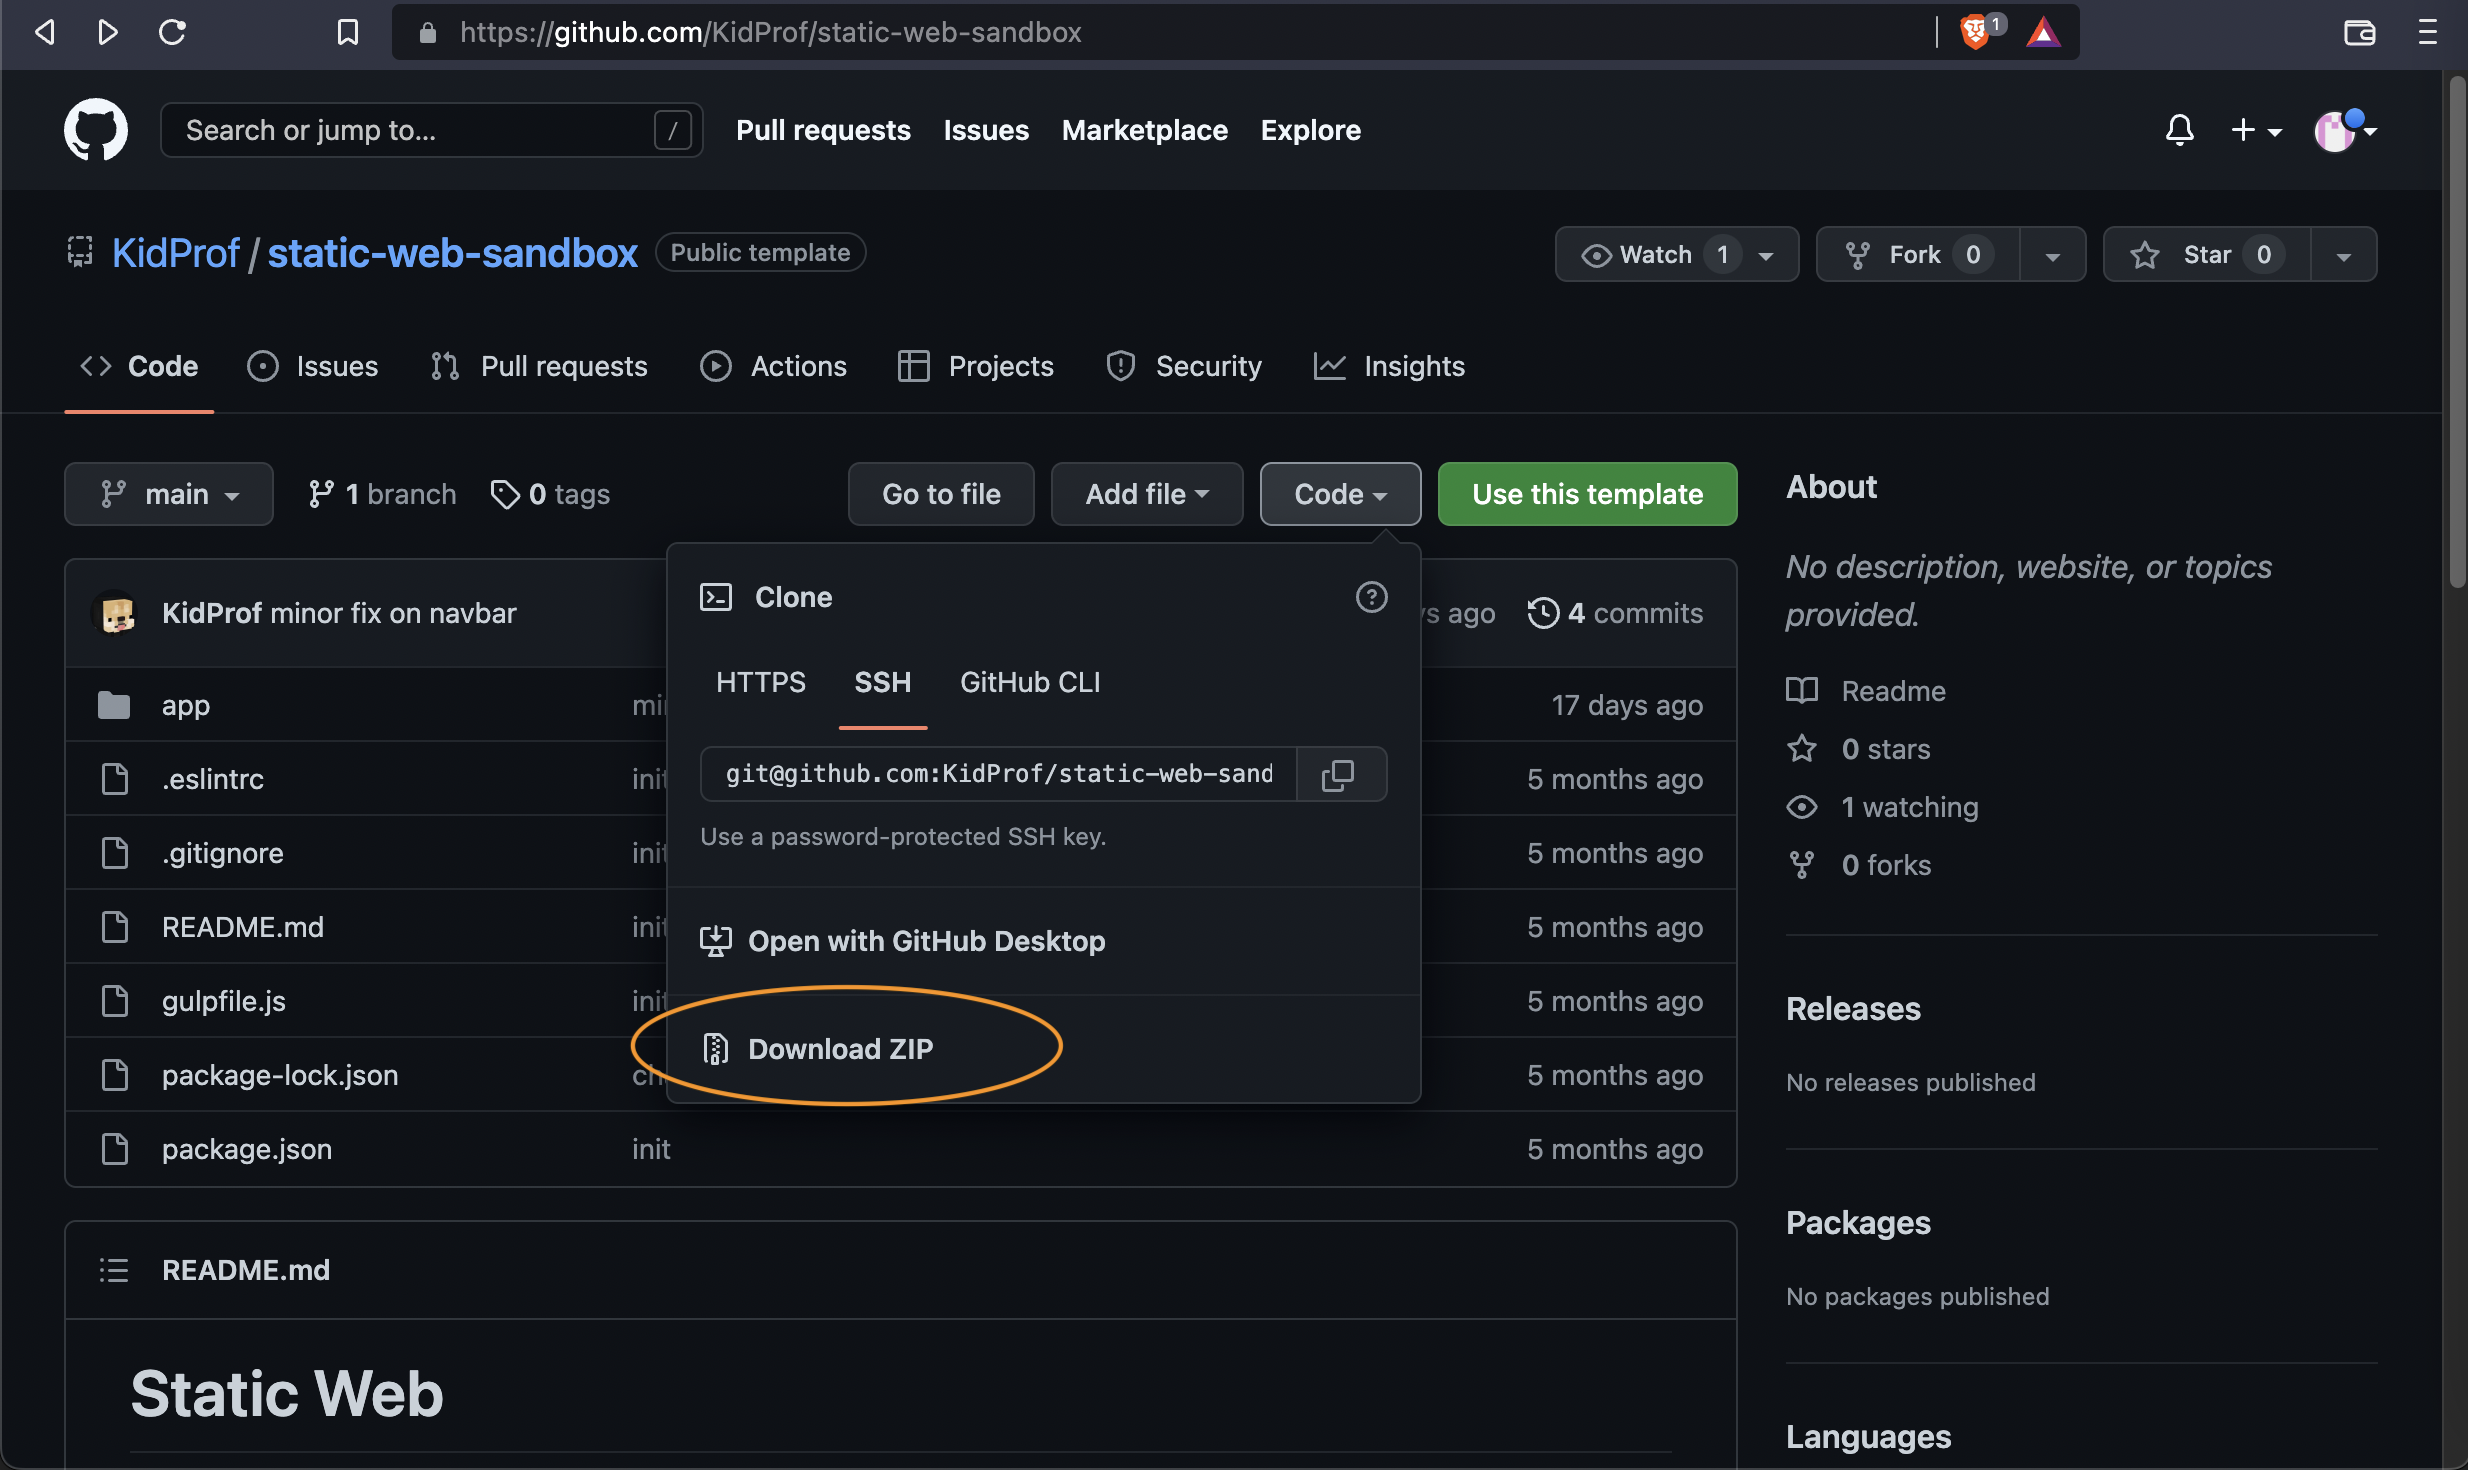
\includegraphics[width=15cm]{images/ch1-download-as-zip.png}
\caption{Screenshot from GitHub showing how to download the code by zip}
\end{figure}


\section{Git Bash (for Windows only)}

\textit{If you are using MacOS or Linux, skip to step 2: Creating a GitHub account}
\vspace{6mm}

Download Git Bash by following \href{https://git-scm.com/download/win}{this link}.\footnote{Link: \href{https://git-scm.com/download/win}{https://git-scm.com/download/win}} It should be straightforward.

\section{Creating a GitHub account}

Create your own GitHub account \href{https://github.com/}{here}.\footnote{Link: \href{https://github.com/}{https://github.com/}} It should be straightforward. Remember the email you used for registration.

\section{Creating a new repository using the template}

Open my template by following \href{https://github.com/KidProf/static-web-sandbox}{this link}.\footnote{Link: \href{https://github.com/KidProf/static-web-sandbox}{https://github.com/KidProf/static-web-sandbox}} Then click the big green button \textit{Use this template}. You will be prompted to create a new repository. \textbf{Repository is a fancier word for project, sometimes abbreviated to repo.} Provide a repository name (a.k.a. project name) of your choice, preferably something meaningful; and you can set it either to public or private based on your own preference. You can change these two settings in the future. Do not change up any other settings in this page. \textit{(see figure)}

\begin{figure}[h]
\centering
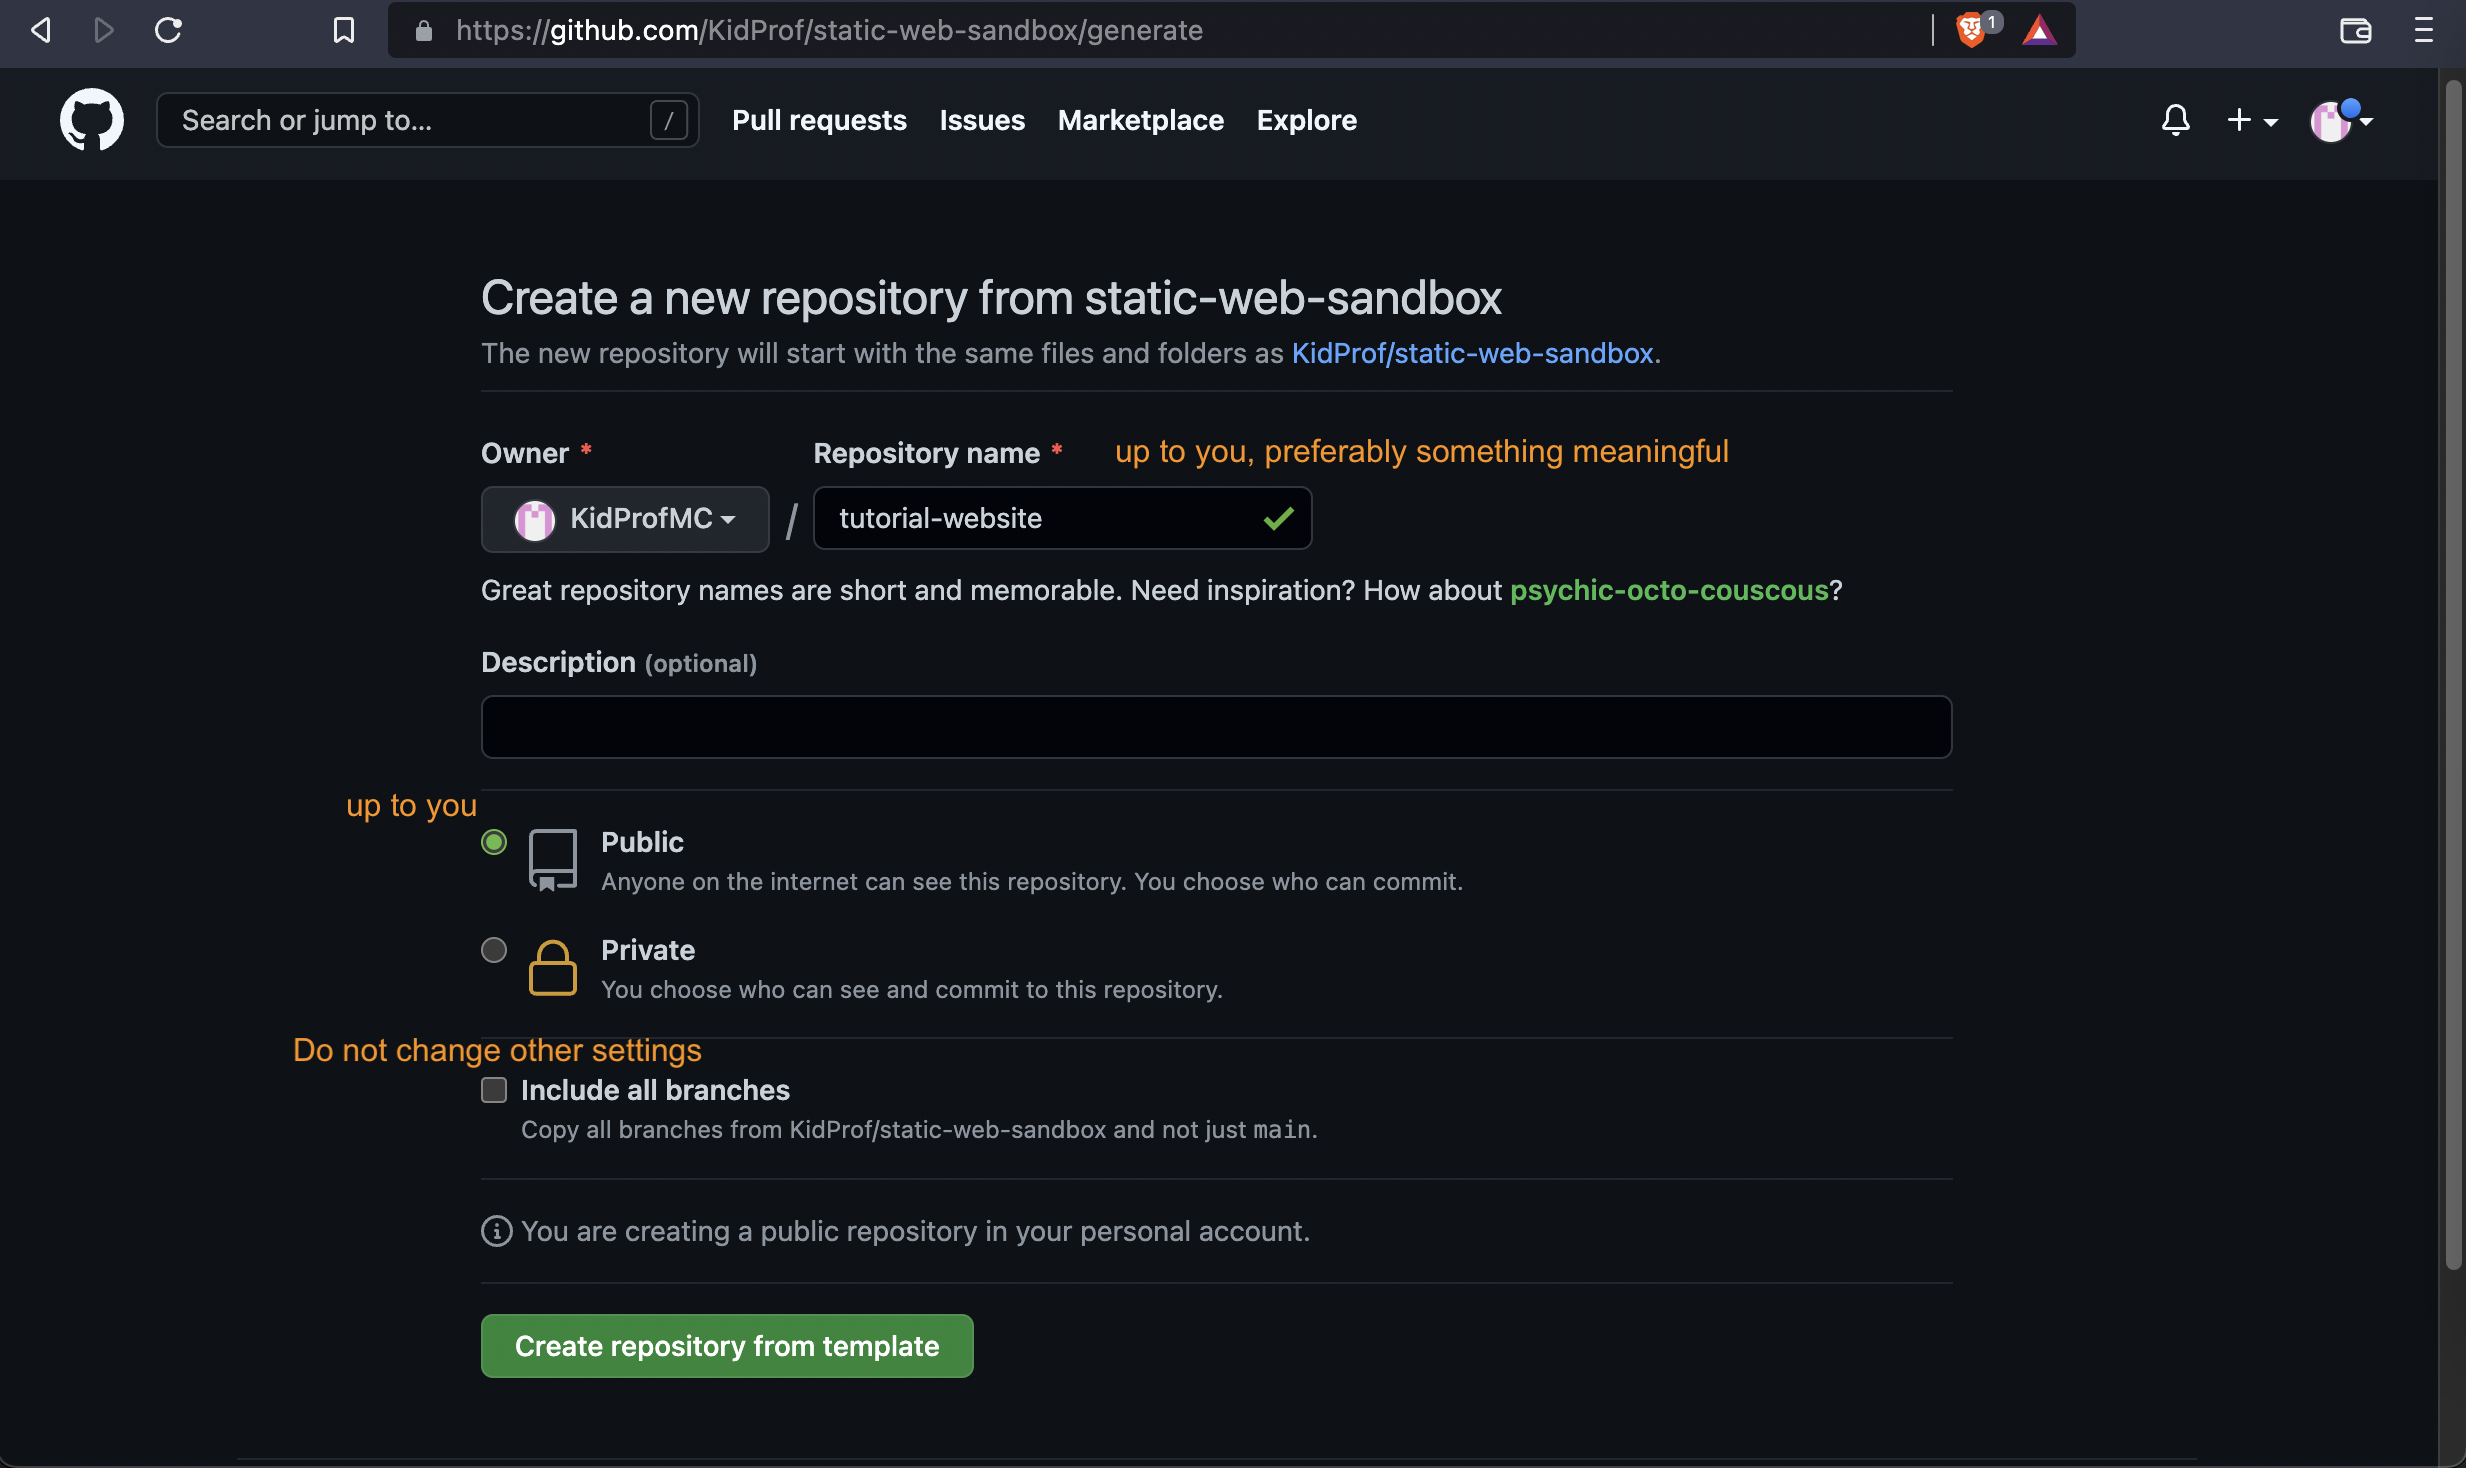
\includegraphics[width=15cm]{images/ch1-create-new-repo.png}
\caption{Creating a new repository}
\end{figure}

\section{Creating an SSH key}

An SSH key is to verify your identity on your local machine, so that you can access and manage your repositories on GitHub from your local machine.

Follow \href{https://docs.github.com/en/authentication/connecting-to-github-with-ssh/generating-a-new-ssh-key-and-adding-it-to-the-ssh-agent}{this tutorial}\footnote{Link: \href{https://docs.github.com/en/authentication/connecting-to-github-with-ssh/generating-a-new-ssh-key-and-adding-it-to-the-ssh-agent}{https://docs.github.com/en/authentication/connecting-to-github-with-ssh/generating-a-new-ssh-key-and-adding-it-to-the-ssh-agent}}, then \href{https://docs.github.com/en/authentication/connecting-to-github-with-ssh/adding-a-new-ssh-key-to-your-github-account}{this tutorial}\footnote{Link: \href{https://docs.github.com/en/authentication/connecting-to-github-with-ssh/adding-a-new-ssh-key-to-your-github-account}{https://docs.github.com/en/authentication/connecting-to-github-with-ssh/adding-a-new-ssh-key-to-your-github-account}}, and you are good to go. 
\vspace{6mm}

Use Git Bash if you are on a Windows machine, use the Terminal if you are on a MacOS or Linux machine. There is no need to understand and remember the commands, copying and pasting is one of the skills needed to be a good programmer. \textbf{The \$ symbol indicates the start of a command, so you do not need to copy it again.}
\vspace{6mm}

For example, if I am using a Windows machine, I would run the following set of commands in my Git Bash line by line. Remember replace the email with your own email used to register for the GitHub account!

\begin{lstlisting}[language=bash]
$ ssh-keygen -t ed25519 -C "your_email@example.com"
$ eval "$(ssh-agent -s)"
$ ssh-add ~/.ssh/id_ed25519
$ clip < ~/.ssh/id_ed25519.pub
\end{lstlisting}

Then paste the SSH public key to the appropriate spot on the GitHub website according to the tutorials.

\section{Creating a folder using command line}

\section{Downloading the code using SSH key}

\section{Installing node.js}

\section{Installing dependencies for the project}

\section{Installing VS Code}